% Tikz File 'topology_details.tex'
\documentclass{standalone}
\usepackage[dvipsnames]{xcolor}
\usepackage{tikz,amsmath,amssymb}
\usepackage[dvipsnames]{xcolor}
\usepackage{tikz}
\usetikzlibrary{arrows,snakes,backgrounds,matrix,patterns,positioning,fadings}
\usepackage{standalone}
\usepackage{subfig}
\usepackage{upgreek}
\usepackage{nicefrac}
\usepackage{dsfont}
\usepackage{bm}
\usepackage{cancel}
\usepackage{amsbsy}
\usepackage{algorithm}
\usepackage{algpseudocode}
\usepackage{lipsum}
\usepackage{harpoon}
\usepackage{comment}
\newenvironment{note}
 {\par\textcolor{Blue}{\bfseries Note:} \color{Blue}\ignorespaces}
 {\par}
\newenvironment{attention}
 {\par\textcolor{red}{\bfseries Attention:} \color{red}\ignorespaces}
 {\par}
\usepackage{hyperref}
\hypersetup{
	colorlinks,
	linkcolor={blue!80!black},
	citecolor={blue!80!black},
	urlcolor={blue!80!black}
}

\newcommand{\mtxb}[1]{\bm{\mathrm{#1}}}
\newcommand{\T}{{\mathrm{T}}}
\newcommand{\herm}{{\mathrm{H}}}
\newcommand{\ev}[1]{\mathrm{E} \left\lbrace #1 \right\rbrace}
\usetikzlibrary{arrows,snakes,backgrounds}
\begin{document}
    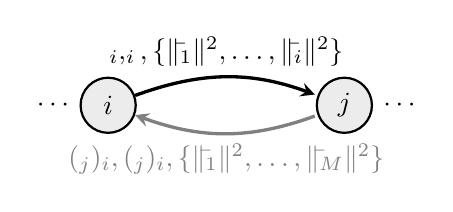
\begin{tikzpicture}[->,shorten >=1pt,auto,semithick, scale=1]
        \tikzstyle{admmnode}=[
            circle,
            draw=black,
            thick,
            text=black,
            minimum size=0.7cm
        ]

        \node[] (C)  at (-2.2,0){\(\cdots\)};

        \node[admmnode, fill=gray!15] (A) at (-1.5,0){\(i\)};
        % \node[draw,text centered] at (-3,-1){\(\mathcal{T}_i = \{\ldots,j,\ldots\}\)};

        \node[admmnode, fill=gray!15] (B) at (1.5,0){\(j\)};
        % \node[draw,text centered] at (3,-1){\(\mathcal{R}_j = \{\ldots,i,\ldots\}\)};

        \node[] (D)  at (2.2,0){\(\cdots\)};
        
        \draw[-stealth,black, line width=1.2] (A) to[bend left=20] node[above, pos=0.5, sloped, scale=1]{\(\x_i, \hf_i, \{\|\bar{\hf}_1\|^2,\ldots,\|\bar{\hf}_i\|^2\}\)}  (B);

        \draw[stealth-,gray, line width=1.2] (A) to[bend right=20] node[below, pos=0.5, sloped,scale=1]{\((\wf_j)_i,(\uuf_j)_i,\{\|\bar{\hf}_1\|^2,\ldots,\|\bar{\hf}_M\|^2\}\)}  (B);
        
    \end{tikzpicture}
\end{document}